\hal{i'm having a hard time understanding what's new and what's prior work here.}

For a typical deep learning model of extractive 
summarization there are two main design decisions:
%At a high level, all the models considered in this paper share the same two part structure: 
\textit{i)}  the choice of \textit{sentence encoder} 
which maps each sentence \sent[i] 
%(treated as a sequence of word embeddings) 
to an embedding $\sentEmb[i] \in \mathcal{R}^{\sentEmbSize}$, 
%\hal{notation class, you used $d$ already for number of sentences} 
and 
\textit{ii)} the choice of \textit{sentence extractor} 
which maps a sequence of sentence embeddings 
$\sentEmb = \sentEmb[1],\ldots, \sentEmb[\docSize]$  
to a sequence of extraction
decisions $\slabel = \slabel_1,\ldots,\slabel_{\docSize}$.
The sentence extractor is then a discriminative 
classifier $p(\slabel | \sentEmb)$.
%and predicts which sentences to extract to produce the 
%extract summary. 

We study three architectures for the sentence encoders, namely, 
embedding averaging, RNNs, and 
CNNs.
We also propose two simple models for the sentence extractor and compare
to the previously proposed extractors of 
\citet{cheng2016neural} and \citet{nallapati2017summarunner}.
The prior works differ significantly but make the same semi-Markovian
factorization of the extraction decisions, i.e. 
$p(\slabel|\sentEmb)=\prod_{i=1}^\docSize p(\slabel[i]|\slabel[<i],\sentEmb)$,
where each prediction \slabel[i] is dependent on all previous \slabel[j] for
all $j < i$.
By contrast, our extractors make a stronger conditional independence 
assumption $p(\slabel|\sentEmb)=\prod_{i=1}^\docSize p(\slabel[i]|\sentEmb)$,
essentially making independent predictions conditioned on $\sentEmb$.
In theory, our models should perform worse because of this, however, as
we later show, this is not the case empirically.






%Depending on the architectural choices of each component we propose we 
%can recover the specific implementations of \cite{cheng&lapata} and 
%\cite{nallapati}, which we outline below.

\subsection{Sentence Encoders}
\begin{figure}
  \center
  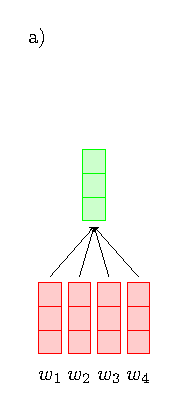
\includegraphics[scale=.7]{figures/avgsentencoder.pdf}
  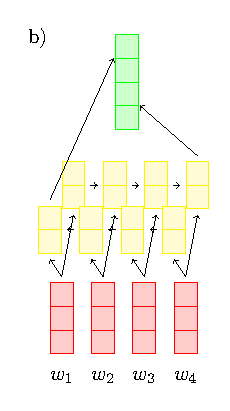
\includegraphics[scale=.7]{figures/rnnsentencoder.pdf}
  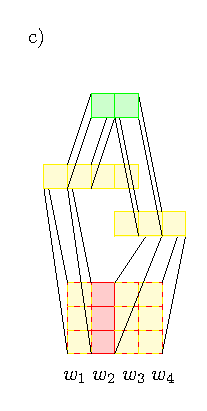
\includegraphics[scale=.7]{figures/cnnsentencoder.pdf}
  \caption{Sentence encoder architectures: a) averaging encoder, b) RNN encoder
           c) CNN encoder. Red indicates word embeddings, yellow indicates
           RNN hidden states or convolutional activations, and green 
           indicates the sentence embedding that is passed to the extractor
           module.}
    \label{fig:encoders}
\end{figure}

We treat each sentence $\sent = \{\wemb_1, \ldots, \wemb_{|\sent|}\}$ 
as a sequence of word embeddings, where $|\sent|$ is the total number of words
in the sentence. We experiment with three architectures for mapping sequences
of word embeddings to a fixed length vector: average pooling, RNNs, and CNNs.
See Figure~\ref{fig:encoders} for a diagram of the three encoders.

\textbf{Averaging Encoder} The averaging encoder (\textit{AVG}) is the simplest
method and has the added benfit of being parameter free. 
A sentence encoding is simply the average of its word embeddings: 
$\operatorname{enc}(\sent) = \frac{1}{|\sent|} \sum_{\wemb \in \sent} \wemb$.


\textbf{RNN Encoder} The \textit{RNN} sentence encoder uses the concatenation 
of the
final output states of a forward and backward RNN over the sentence's word
embeddings. We use a Gated Recurrent Unit (GRU) \cite{cho} for the RNN cell,
since it has fewer parameters than the equivalent LSTM but with similar 
performance. Formally, an \textit{RNN} sentence encoding is defined as
$\operatorname{enc}(s) = [\rSentVec_{|\sent|}; \lSentVec_1]$
where 
\begin{align} 
\rSentVec_i &= \rgru(w_i, \rSentVec_{i-1}) \\
\lSentVec_i &= \lgru(w_i, \lSentVec_{i+1}) 
\end{align}
for all $i \in 1, \ldots, |\sent|$. $\rgru$ amd $\lgru$ indicate the 
forward and backward GRUs respectively, and each have separate learned 
parameters.
The initial states $\rSentVec_0$ and $\lSentVec_{\sentSize + 1}$ are not 
learned and are set to zero vectors.

\textbf{CNN Encoder} The \textit{CNN} sentence encoder uses a series of 
convolutional feature maps to encode each sentence. This encoder is similar
to the convolutional architecture of \cite{kim} used for text classification
tasks and performs a series of ``one-dimensional'' convolutions over 
word embeddings. 
The \textit{CNN} encoder has hyperparameters
associated with the window sizes $\maxWindowSize \subset \mathcal{N}$ of the convolutional filter 
(i.e. the number of words associated with each convolution) and the number of 
feature maps $\maxFeatureMaps$ associated with each filter
(i.e. the output dimension of each 
convolution). 
The \textit{CNN} sentence encoding is computed as follows:
\begin{align}
 \specActivation_i &= \specConvBias 
    + \sum^\filterWindowSize_{j=1} \specConvWeight_j \cdot \wemb_{i + j -1}\\
  \specFeatureMap &= \max_{i\in 1,\dots, |\sent| - \filterWindowSize + 1} 
                      \relu\left(\specActivation_i\right) \\
 \senc(s) &= \left[\specFeatureMap | 
   \numFeatureMaps \in \{1, \ldots, \maxFeatureMaps\},
   \filterWindowSize \in \maxWindowSize
   \right]
\end{align}
where $\specConvBias\in\mathcal{R}$ and $\specConvWeight \in 
\mathcal{R}^{\filterWindowSize \times \wembdim}$ are learned bias and filter
weight parameters respectively, and $\relu(x) = \max(0, x)$ is the rectified
linear unit \cite{relu}.




\subsection{Sentence Extractors}
\begin{figure*}
  \center
  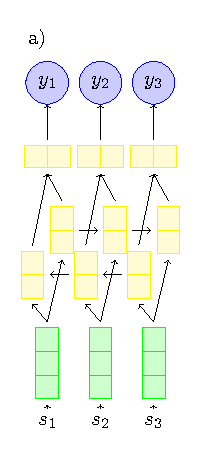
\includegraphics[scale=.7]{figures/rnnextractor.pdf}
  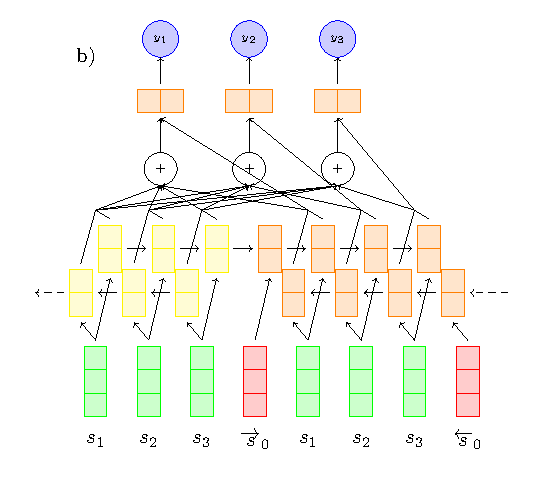
\includegraphics[scale=.7]{figures/s2s_extractor.pdf}
  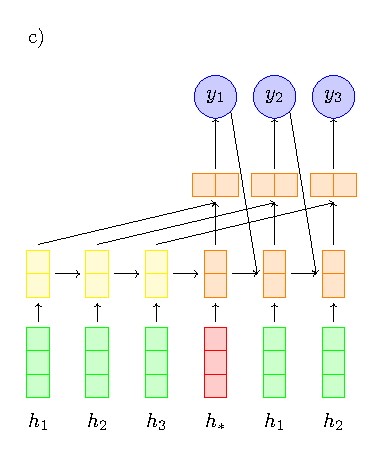
\includegraphics[scale=.7]{figures/clextractor.pdf}
  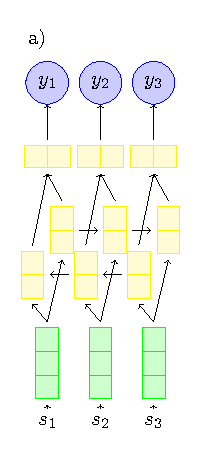
\includegraphics[scale=.7]{figures/rnnextractor.pdf}
  \caption{Sentence extractor architectures: a) \modelOneBF, b) \modelTwoBF,
            c) \baselineOneBF, and d) \baselineTwoBF. }
  \label{fig:extractors}
\end{figure*}

Given a sequence of sentence embeddings $\sentvec_i = \senc(\sent_i)$,
a sentence extractor produces a conditional distribution over the 
corresponding sentence extraction variables 
$p(\slabel_1,\ldots,\slabel_{\sentSize}|\sentvec_1, \ldots, \sentvec_{\sentSize})$.
We propose two simple recurrent neural network based sentence extractors
that make a strong conditional independence assumption over the labels
$\slabel_i$, namely
$\explicitLikelihood= \naiveLikelihood$. This stands in contrast to our 
baseline models which make a weaker assumption, \hal{this is really confusing cuz i don't think you've specified this yet, and it's still hard to understand what's new/yours and what's old/baseline.}
$\compactLikelihood = \markovLikelihood$, at the expense of greater 
computational complexity. See Figure~\ref{fig:extractors} for a diagram of the 
four sentence extractor architectures.

\textbf{RNN Extractor} Our first proposed model is a very simple bidirectional
RNN based tagging model. As in the RNN sentence encoder we use a GRU cell.
The the forward and backward outputs of each sentence are passed through a 
single layer perceptron with a logsitic sigmoid output (denoted by $\sigma$)
to predict the probability
of extracting each sentence:
\hal{i'd sugest following the same notation as before to remove the zero comment}
\begin{align}
    \rExtHidden_i &= \rgru(\sentvec_i, \rExtHidden_{i-1}) \\
   \lExtHidden_i &= \lgru(\sentvec_i, \lExtHidden_{i+1}) \\
   \logits_i &= \relu\left(U \cdot [\rExtHidden_i; \lExtHidden_i] + u \right)\\
   p(\slabel_i=1|\sentvec) &= \sigma\left(V\cdot \logits_i + v  \right)
\end{align}
for all $i \in 1, \ldots, \docsize$. $\rgru$ amd $\lgru$ indicate the 
forward and backward GRUs respectively, and each have separate learned 
parameters; $U, V$ and $u, v$ are learned weight and bias parameters.
\textcolor{red}{The initial states $\rExtHidden_0$ and $\lExtHidden_{\docsize + 1}$ are not 
learned and are set to zero vectors.}



\textbf{\sts~Extractor} One shortcoming of the RNN extractor is that long range
information from one end of the document may not easily be able to effect 
extraction probabilities of sentences at the other end. 
Our second proposed model, which we refer to as the \stsbf~extractor,
is based on the attentional sequence-to-sequence models commonly
used for neural machine translation \cite{badhanau} and 
abstractive summarization \cite{see}. The sentence embeddings are first
encoded by a bidirectional $\gru$. A separate decoder $\gru$ transforms each 
sentence into a query vector which attends to the encoder output. The
attention weighted encoder output and the decoder $\gru$ output are concatenated
and fed into a multi-layer percepron to compute the extraction probability.
Formally we have:
\begin{align}
  \rEncExtHidden_i &= \rgru_{enc}(\sentvec_i, \rEncExtHidden_{i-1}) \\
  \lEncExtHidden_i &= \lgru_{enc}(\sentvec_i, \lEncExtHidden_{i+1}) \\
  \rDecExtHidden_i &= \rgru_{dec}(\sentvec_i, \rDecExtHidden_{i-1}) \\
  \lDecExtHidden_i &= \lgru_{dec}(\sentvec_i, \lDecExtHidden_{i+1}) 
\end{align}
\begin{align}
 \decExtHidden_i = [\rDecExtHidden_i; \lDecExtHidden_i], &\;\;
 \encExtHidden_i = [\rEncExtHidden_i; \lEncExtHidden_i] 
\end{align}
\begin{align}
 \alpha_{i,j} = 
   \frac{\exp \left(\decExtHidden_i \cdot \encExtHidden_j \right)}{
   \sum_{j=1}^{\docsize}\exp\left(\decExtHidden_i \cdot \encExtHidden_j\right)}, 
& \;\; \attnExtHidden_i = \sum_{j=1}^{\docsize} \alpha_{i,j} \encExtHidden_j 
\end{align}
\begin{align}
   \logits_i = \relu\left(U \cdot [\attnExtHidden_i; \decExtHidden_i] + u \right)&\\
   p(\slabel_i=1|\sentvec) = \sigma\left(V\cdot \logits_i + v  \right),
\end{align}
for all $i \in 1, \ldots, \docsize$.
The final outputs of each encoder direction are passed to first decoder
steps; additionally, the first step of the decoder GRUs are learened 
``begin decoding'' vectors $\rDecExtHidden_0$ and $\lDecExtHidden_0$ (
see Figure~\ref{fig:extractors}.b).
Each GRU has separate learned 
parameters; $U, V$ and $u, v$ are learned weight and bias parameters.
\textcolor{red}{The initial states $\rExtHidden_0$ and $\lExtHidden_{\docsize + 1}$ are not 
learned and are set to zero vectors.}


\textbf{Cheng \& Lapata Extractor} 
We compare the previously proposed architectures to the sentence extractor
model of \cite{chenglapata}. Unlike the previous models where
sentence extraction predictions are conditionally independent given
the sentence embeddings, this model uses previous extraction probabilities to
influence later decisions. The basic architecture is a unidirectional
sequence-to-seqeunce
model defined as follows:
\begin{align}
    \encExtHidden_i &= \gru_{enc}(\sentvec_i, \encExtHidden_{i-1}) \\
    \decExtHidden_i &= \gru_{dec}(p_{i-1} \cdot \sentvec_{i-1}, \decExtHidden_{i-1}) \\
   \logits_i &= \relu\left(U \cdot [\encExtHidden_i; \decExtHidden_i] + u \right)\\
    p_i &= p(\slabel_i=1|\slabel_{<i}, \sentvec) = \sigma\left(V\cdot \logits_i + v  \right) 
\end{align}
for all $i \in 1, \ldots, \docsize$.
The final output of the encoder is passed to the first decoder
step; additionally, the first step of the decoder GRU is a learned 
``begin decoding'' vector $\decExtHidden_0$ (
see Figure~\ref{fig:extractors}.c).
Each GRU has separate learned 
parameters; $U, V$ and $u, v$ are learned weight and bias parameters.
\textcolor{red}{The initial states $\rExtHidden_0$ and $\lExtHidden_{\docsize + 1}$ are not 
learned and are set to zero vectors.}
 Note in \textcolor{red}{Equation 18} that 
the decoder side GRU input is the sentence embedding from the previous time
step weighted by its probabilitiy of extraction ($p_{i-1}$) from the 
previous step.

We refer to this extractor as the \baselineOneBF~extractor; the model 
architecture descrbied in \cite{cl} is equaivalent to the
\baselineOneBF~extractor paired with the \textit{CNN} encoder.

\hal{i'd use full names throughout if possible, so just \textbf{Chang\&Lapata} and \textbf{SummaRunner} and...}

\textbf{SummaRunner Extractor}
Our second baseline extractor is taken from \cite{nallapati}, which like the
\modelOneBF~extractor starts with a bidrectional GRU over the sentence 
embeddings 
\begin{align}
  \rEncExtHidden_i &= \rgru(\sentvec_i, \rEncExtHidden_{i-1}) \\
  \lEncExtHidden_i &= \lgru(\sentvec_i, \lEncExtHidden_{i+1}),
\end{align}
for all $i \in 1,\ldots,\docsize$. 
\textcolor{red}{The initial states $\rExtHidden_0$ and $\lExtHidden_{\docsize + 1}$ are not
learned and are set to zero vectors.}


Unlike \modelOneBF, however, it then creates a representation
of the whole document $q$ by passing the averaged GRU output states through
a fully connected layer: 
\begin{align}
q = \tanh\left(b_q + W_q\frac{1}{\docsize}\sum_{i=1}^{\docsize} [\rEncExtHidden_i; \lEncExtHidden_i] \right)
\end{align}
A concatentation of the GRU outputs at each step
are passed through a separate fully connected layer to create a 
sentence representation $z_i$, where
\begin{align}
    \extHidden_i &= \relu\left(b_z + W_z [\rEncExtHidden_i; \lEncExtHidden_i]\right).
\end{align}
The extraction probability is then determined by contributions from five 
sources,
\textit{i)} a content score $a^{(con)}_i=W_{con}\cdot z_i$, 
\textit{ii)} a salience score $a^{(sal)}_i = z_i^TW_{sal} \cdot q$ quantifying the 
similarity of the sentence to the document, 
\textit{iii)} a novelty score $a^{(nov)}_i = -z_i^TW_{nov} \cdot \tanh(g_i)$
that tracks negative similarity to a representation of the extract summary 
$g_i$,
\textit{iv)} a fine-grained position score 
$a^{(fpos)}_i = W_{fpos}\cdot p_i$ where
$p_i$ is a sentence position embedding for the $i$-th position in the document,
and \textit{v)} a coarse-grained position score 
$a^{(cpos)}_i = W_{cpos}\cdot r_i$ where
$r_i$ is a position embedding for the quarter of the document
that sentence $i$ occurs in.
The final extraction probability is the logistic sigmoid of the
sum of these terms plus a bias,
\begin{align}
    p(y_i=1|y_{<i}, h) &= \sigma\left(\begin{array}{l}
      a_i^{(con)} + a_i^{(sal)} + a_i^{(nov)} \\
  + a_i^{(fpos)}  + a_i^{(cpos)} + b \end{array}\right).
\end{align}
Finally, the iterative summary representation $g_i$ is computed as a 
sum of the previous $z_{<i}$ weighted by their extraction probabilities,
\begin{align}
g_i & = \sum_{j=1}^{i-1} p(y_j=1|y_{<j},h) \cdot z_j.
\end{align}
Note that the presence of this term induces dependence of each $y_i$ to 
all $y_{j}$ for $j < i$ similarly to the \baselineOneBF~extractor.
The combination of this extractor, which we refer to as $\baselineTwoBF$,
and the \textit{RNN} encoder is most similar to the architecture described 
in \cite{nallapati} with the principal difference that we are using the RNN
final states for the sentence representation and they used the average of
the RNN output.

%\begin{align}
%    \extHidden_i &= \relu\left(b_z + W_z [\rEncExtHidden_i; \lEncExtHidden_i]\right)
%  \end{align}
%  \begin{align*}
%      p(y_i=1|y_{<i}, h) = \sigma(& W_{con}\cdot z_i \\
%                     & + z_i^T W_{sal}\cdot q \\
%                     & -z_i^T W_{nov} \cdot \tanh(g_i) \\
%                     & + b_{rp_i}  \\
%                     & + b_{ap_i} \\
%                     & + b)     \\
%      g_j & = \sum_{i=1}^{j-1} p(y_j=1|y_{<j},h) \cdot z_j
%\end{align*}



%%% Local Variables:
%%% mode: latex
%%% TeX-master: "dlextsum.emnlp18"
%%% End:



%%% Local Variables:
%%% mode: latex
%%% TeX-master: "dlextsum.emnlp18"
%%% End:
